%----------------------------------------------------------------------
%	REQUIRED PACKAGES
%----------------------------------------------------------------------
\documentclass[12pt]{report}
\usepackage[numbers,sort&compress]{natbib}
\usepackage[utf8]{inputenc}
\usepackage{amsmath,amsfonts,amssymb}
\usepackage{graphicx}
\usepackage{tikz}
\usepackage{float}
\usepackage{placeins}
\usepackage{url}
\usepackage{caption}
\usepackage{setspace}
\usepackage{tocloft}
\usepackage{cite}


%----------------------------------------------------------------------
%	FONTS,INDENTATION, MARGINS, LINE SPACING
%----------------------------------------------------------------------
\usepackage{times}      % Loads the Times-Roman Fonts
\usepackage{mathptmx}   % Loads the Times-Roman Math Fonts
\usepackage[left=3.81cm,
            right=2.54cm,
		top=2.54cm,
		bottom=2.54cm,
		a4paper]{geometry}
  
\setlength{\parindent}{0pt} % Remove paragraph indent globally
\usepackage{setspace} %package for line spacing
\setstretch{1.5}
\usepackage{parskip}
\setlength{\parskip}{6pt}  % Adjust paragraph spacing as needed

%----------------------------------------------------------------------
%	TITLES,SECTIONS,SUBSECTIONS AND SUBSUBSECTIONS
%----------------------------------------------------------------------
\usepackage{titlesec}
\titlespacing{\chapter}{0pt}{-24pt}{12pt}
\titlespacing{\section}{0pt}{16pt}{16pt}
\titlespacing{\subsection}{0pt}{16pt}{16pt}
\titlespacing{\subsubsection}{0pt}{16pt}{16pt}

\titleformat{\chapter}[display]{\centering\fontsize{14pt}{12pt}\bfseries}{\MakeUppercase{\chaptertitlename\ \thechapter}}{12pt}{}
\titleformat{\section}{\fontsize{12pt}{16pt}\bfseries\raggedright}{\thesection}{0.5em}{}
\titleformat{\subsection}{\fontsize{12pt}{16pt}\bfseries\raggedright}{\thesubsection}{0.5em}{}
\titleformat{\subsubsection}{\fontsize{12pt}{16pt}\bfseries\raggedright}{\thesubsubsection}{0.5em}{}
\titleformat{\paragraph}{\fontsize{12pt}{0pt}\bfseries\raggedright}{\theparagraph}{0.5em}{}

%----------------------------------------------------------------------
%	FORMATTING THE TABLE OF CONTENTS,LOF AND LOT
%----------------------------------------------------------------------

% Adjust the spacing for the TABLE OF CONTENT
\renewcommand{\cftbeforetoctitleskip}{-18pt} % Space before the TOC title
\renewcommand{\cftaftertoctitleskip}{12pt} % Space after the TOC title
\renewcommand{\cftbeforechapskip}{9pt} % Space before each chapter entry
\renewcommand{\cftbeforesecskip}{9pt} % Space before each section entry
\renewcommand{\cftbeforesubsecskip}{9pt} % Space before each section entry
\renewcommand{\contentsname}{\fontsize{14}{16}\bfseries TABLE OF CONTENTS}

% Adjust the spacing for the LIST OF FIGURES
\renewcommand{\cftbeforeloftitleskip}{-18pt} % Space before the LOF title
\renewcommand{\cftafterloftitleskip}{12pt} % Space after the LOF title
\renewcommand{\cftbeforefigskip}{10pt} % Space before each figure entry
\renewcommand{\listfigurename}{\fontsize{14}{16}\bfseries LIST OF FIGURES}
\renewcommand{\cftfigpresnum}{\figurename\ }
\renewcommand{\cftfigaftersnum}{:}
\renewcommand{\cftfigaftersnumb}{\hspace{2.5em}} 

% Adjust the spacing for the LIST OF TABLES
\renewcommand{\cftbeforelottitleskip}{-18pt} % Space before the LOT title
\renewcommand{\cftafterlottitleskip}{12pt} % Space after the LOT title
\renewcommand{\cftbeforetabskip}{10pt} % Space before each table entry
\renewcommand{\listtablename}{\fontsize{14}{16}\bfseries LIST OF TABLES}
\renewcommand{\cfttabpresnum}{Table\ }
\renewcommand{\cfttabaftersnum}{:}
\renewcommand{\cfttabaftersnumb}{\hspace{2.5em}}

%----------------------------------------------------------------------
%	END OF PREAMLBE AND BEGINNING OF THE DOCUMENT
%----------------------------------------------------------------------

\begin{document}

\pagenumbering{roman} % roman page numbers
\begin{titlepage}
    \centering
    
    
\includegraphics[width=0.2\textwidth]{Graphics/TULogo.png}\par
    \vspace{1.2cm}
    {\fontsize{14pt}{12pt}\selectfont\bfseries\textcolor{black}
    TRIBHUVAN UNIVERSITY \par INSTITUTE OF ENGINEERING \par PURWANCHAL CAMPUS \par
    \vspace{1.2cm}
    \begin{flushleft}
    
    \end{flushleft}

    % {\bfseries\textcolor{black}
    \par A MINOR PROJECT PROPOSAL ON
    
    STOCKHAWK : COMPREHENSIVE STOCK TRACKER,PREDICTION AND ALERT PLATFORM\par

    \vspace{1.2cm}
    BY\par SUJIT KUMAR DAS (PUR078BCT091)
      \par SHUVKANT CHAUDHARY PHANAIT (PUR078BCT081)
      \par SNEHA PATEL (PUR078BCT083)
      \par SHYAM KRISHNA GUPTA (PUR078BCT082)
    \par
    \vspace{1.2cm}\par
    }
    {\fontsize{13pt}{12pt}\selectfont\bfseries\textcolor{black}
    DEPARTMENT OF ELECTRONICS AND COMPUTER ENGINEERING\par PURWANCHAL CAMPUS\par DHARAN, NEPAL\par
    \vspace{1.2cm}
    \vspace{1.2cm}
    
     DECEMBER,2024 
    }
\end{titlepage}


%\pagenumbering{roman} % roman page numbers
\begin{titlepage}
    \centering
    
    {\fontsize{12pt}{14pt}\bfseries\textcolor{black}{PROJECT TITLE GOES HERE}\par}
    \vspace{2.0cm}
       {By} \par {STUDENT NAME}({ROLL NUMBER})
            \par {STUDENT NAME}({ROLL NUMBER})
            \par {STUDENT NAME}({ROLL NUMBER})
            \par {STUDENT NAME}({ROLL NUMBER})
       \vspace{2.0cm}\par
    Project Supervisor\par
    Asst. Prof. Pukar Karki\par
    \vspace{2.0cm}
    {A project submitted to the Department of Electronics and Computer Engineering in partial fulfillment of the requirements for the Bachelor’s Degree in Computer Engineering}\par
        \vspace{2.0cm}\par

    {Department of Electronics and Computer Engineering\\ Purwanchal Campus, Institute of Engineering \\ Tribhuvan University\\ Dharan, Nepal}\par
        \vspace{2.0cm}\par
        
   {January , 2024}
   
\end{titlepage}




%\include{Copyright}
%\include{Declaration}
%\chapter*{RECOMMENDATION}
\addcontentsline{toc}{chapter}{RECOMMENDATION}
The undersigned certify that they have read and recommended to the Department of
Electronics and Computer Engineering for acceptance, a project entitled \textbf{``PROJECT NAME GOES HERE"}, submitted by \textbf{STUDENTS NAME} in partial fulfillment of the requirement for the award of the degree of \textbf{``Bachelor of Engineering in Computer Engineering"}.\par
        \vspace{1cm}
..........................................................................\\
\textbf{Asst. Prof. Pukar Karki\\
Supervisor\\
Department of Electronics and Computer Engineering\\
Purwanchal Campus, Institute of Engineering, Tribhuvan University}\par
        \vspace{1cm}
..........................................................................\\
\textbf{Prof. Subarna Shakya, (PhD)\\
External Examiner \\
Department of Electronics and Computer Engineering\\
Pulchowk Campus, Institute of Engineering, Tribhuvan University}\par
        \vspace{1cm}
..........................................................................\\
\textbf{
Asst. Prof. Pravin Sangroula\\ 
Head of Department \\
Department of Electronics and Computer Engineering\\Purwanchal Campus, Institute of Engineering, Tribhuvan University}\par
\vspace{2.5cm}

\begin{center}
\textbf{10\textsuperscript{th} January, 2024}
\end{center}
\newpage


%\include{DeptAcceptance}
\chapter*{ACKNOWLEDGEMENT}
\addcontentsline{toc}{chapter}{ACKNOWLEDGEMENT}
We would like to express our sincere gratitude to the Deputy Head of the Department, Asst. Prof. Pukar Karki for his invaluable guidance, expertise, and unwavering encouragement throughout the course of our minor project proposal. Their support has been instrumental in shaping the direction and success of our research endeavor. 

 We extend our heartfelt gratitude to the Department of Electronics and Computer Engineering at Purwanchal Campus for granting us the opportunity to undertake this project. We also wish to acknowledge our esteemed colleagues, friends, and peers for their enriching interactions and constant inspiration. The incisive feedback, intellectually stimulating discussions, and collaborative spirit from our fellow contributors have elevated the overall quality of our project. 
 Any kind of suggestion or criticism will be greatly appreciated and acknowledged.

\vspace{1cm}




\chapter*{ABSTRACT}
\addcontentsline{toc}{chapter}{ABSTRACT}
This project focuses on developing a comprehensive system for tracking the stock market, predicting future price movements, and notifying users when their predefined goals align with market conditions. By leveraging external APIs for real-time stock data and historical trends, the system employs advanced machine learning algorithms, including LSTM, for price forecasting. It ensures scalability and reliability, with MongoDB managing time-series data and PostgreSQL handling user-related information. The system offers a user-friendly interface for tracking stocks, setting goals, and receiving customized alerts, empowering users to make informed investment decisions efficiently.

\vspace{1cm}

{\centering{\tableofcontents}}\newpage
{\centering\listoffigures\addcontentsline{toc}{chapter}{LIST OF FIGURES}}
\newpage
% {\centering\listoftables\addcontentsline{toc}{chapter}{LIST OF TABLES}}
\newpage
\newpage
\chapter*{LIST OF ABBREVIATIONS}
% \vspace{1cm}
\addcontentsline{toc}{chapter}{LIST OF ABBREVIATIONS}
\begin{tabular}{l l}
API	&	:	Application Programming Interface	\\
LSTM & : Long Short Term Memory\\
ANN & : Artificial Neural Network\\
RNN & : Recurrent Neural Network\\



\end{tabular}









\pagenumbering{arabic}
\chapter{INTRODUCTION}
\section{Background}
The stock market is a crucial part of the global economy, where people and businesses invest to grow their wealth. However, it can be unpredictable and fast-moving, making it difficult for investors to keep up with changes and make the right decisions at the right time. Monitoring market trends, predicting price changes, and identifying the best opportunities require a lot of effort and expertise. By using advanced algorithms, technology can simplify these tasks, helping investors track and understand market patterns more easily and alerting the users when to invest and sell the stocks will help the users to connect with market adequately.



 \section{Problem Statement}
 While there are tools available to analyze the stock market, many of them have limitations. They often lack real-time updates, fail to provide personalized notifications, and do not predict future price movements effectively. These issues make it harder for users to make timely and well-informed decisions.The main problem in predicting share market is that the
share market is a chaos system. There are many variables
that could affect the share market directly or indirectly.
There are no significant relations between the variables and
the price. We cannot draw any mathematical relation
among the variables. There are no laws of predicting the
share price using these variables.
 This gap highlights the necessity for a comprehensive, user-centric platform that not only tracks stock market activity but also empowers users with actionable insights and timely alerts.


\section{Motivation}
The motivation for this project stems from the need to create a comprehensive tool that empowers users by providing real-time market data, customized notifications, and predictive analytics. This ensures that users can make informed choices and achieve their investment goals with greater ease.

\section{Objectives of the Study}

The primary objectives of this program are:
  \begin{enumerate}

\item To estimate future price movements using LSTM algorithm.

\item To alert users when their target prices align with projections.

\item To streamline market tracking by delivering real-time information and personalized insights, enabling users to make smarter investment decisions.
\item To study the risks and challenges of AI in stock market prediction.
  \end{enumerate}



    





\chapter{RELATED THEORY}
\section{Related Theory:}
Stock market analysis relies on a combination of theoretical frameworks and advanced computational techniques. StockHawk incorporates these principles to provide users with a comprehensive tool for monitoring and predicting stock market movements. Below is a discussion of foundational theories in stock market analysis and how they relate to StockHawk’s features and objectives.

\textbf{1. Time-Series Forecasting}

Time-series forecasting is a statistical technique used to analyze and predict future values based on historical data. In stock market analysis, it helps identify trends, seasonality, and cyclic patterns in stock prices.

\textbf{Application in StockHawk:}

StockHawk uses time-series forecasting to estimate future price movements. By leveraging historical stock data and applying algorithms such as ), LSTM - exponential smoothing, and neural networks, the platform generates accurate predictions of future price trends. These predictions empower users to anticipate changes in the market and make informed decisions about buying, selling, or holding their investments.

\textbf{ Objective Alignment:}

To estimate future price movements using advanced algorithms: StockHawk's forecasting capabilities enable users to plan their strategies based on data-driven insights.

\textbf{2. Pattern Recognition}

Pattern recognition involves identifying recurring structures or behaviors in data. In stock market analysis, it is used to detect trends, support and resistance levels, and technical indicators such as head-and-shoulders patterns or moving averages.

\textbf{Application in StockHawk:}

StockHawk integrates pattern recognition techniques to track stock market patterns effectively. Machine learning models and technical analysis tools help identify significant market signals, allowing users to understand the broader market dynamics and make timely decisions.

\textbf{Objective Alignment}:

To track stock market patterns effectively: By recognizing key patterns, StockHawk simplifies complex market data into actionable insights.

\textbf{3. Real-Time Data Processing and Alerts}

In today’s fast-paced markets, real-time information is crucial. Technologies like data streaming, API integration, and low-latency systems enable platforms to deliver updates almost instantly.

\textbf{
Application in StockHawk:}

StockHawk provides real-time data and personalized alerts. By continuously monitoring market conditions, it notifies users when their target prices match projections. This feature ensures that users never miss critical opportunities, enhancing their ability to act promptly.

\textbf{Objective Alignment:}

To alert users when their target prices align with projections: Real-time alerts are tailored to each user’s goals, keeping them informed and prepared to act.
To streamline market tracking by delivering real-time information and personalized insights: The platform’s ability to process and display real-time data ensures users can rely on up-to-date information for decision-making.

\textbf{4. Behavioral Finance and Decision-Making Support}

Behavioral finance examines the psychological influences on investors’ decisions, such as fear, greed, and overconfidence. Recognizing these biases helps design systems that guide users toward rational decision-making.

\textbf{Application in StockHawk:}

By offering clear, data-driven insights and removing the noise of irrelevant information, StockHawk supports users in making smarter investment choices. Personalized insights help users overcome emotional biases and focus on objective analysis.

\textbf{Objective Alignment:}

To streamline market tracking by delivering real-time information and personalized insights: StockHawk’s intuitive interface and insights reduce cognitive overload, making complex information more accessible and actionable.




\chapter{LITERATURE REVIEW}
\section{ Introduction}
Stock market tracking and prediction tools have become essential for investors seeking to make informed decisions in a fast-moving and unpredictable market. Numerous platforms exist that claim to help users predict price movements and track trends, but each has its own strengths and weaknesses. This section reviews the existing tools and highlights their limitations, explaining how StockHawk addresses these gaps.

\subsection {Traditional Stock Market Tracking Tools}

Traditional stock market tracking tools, such as Yahoo Finance, Google Finance, and Bloomberg, provide basic functionalities like real-time stock price tracking, historical data analysis, and financial news. These platforms typically focus on displaying data and offering some basic charting features.

% \textbf{Limitations:}
% While these tools are useful for observing current market data, they lack advanced prediction capabilities. They do not provide personalized alerts or predictive analytics that are tailored to individual user goals. Additionally, they focus mainly on historical data and do not offer real-time, actionable insights based on current market conditions.

% \textbf{How StockHawk Addresses the Gap:}
% StockHawk goes beyond traditional tracking by offering personalized, real-time alerts when target prices align with predicted price movements. The platform’s advanced algorithms help estimate future price trends, making it a powerful tool for proactive decision-making. Unlike traditional tools that focus primarily on price history, StockHawk enables users to anticipate market shifts before they occur.


\subsection {Machine Learning and AI-Based Tools}

More advanced platforms like TrendSpider and Kavout use machine learning and AI algorithms to predict future stock prices. These platforms attempt to automate the analysis of stock trends by applying deep learning models to large datasets.

% \textbf{Limitations:}
% While machine learning-based tools are capable of making predictions, they can be opaque in terms of how decisions are made. Many AI-based platforms lack transparency, making it difficult for users to understand the rationale behind predictions. Additionally, these systems can be computationally expensive, and their results may not always be accessible to non-expert users.

% \textbf{How StockHawk Addresses the Gap:}
% StockHawk integrates advanced algorithms for price prediction in a user-friendly interface, making it more accessible to a wider range of users, from beginners to experts. The platform is designed to offer transparency and clarity in its predictions, with clear explanations of the reasoning behind the alerts and projections. Moreover, StockHawk focuses on providing personalized insights and real-time updates, ensuring users receive relevant information tailored to their investment goals.

% \section{ Limitations of Existing Tools and StockHawk’s Advantages}

% The major \textbf{limitations }of current stock tracking and prediction tools are:

% A lack of personalized alerts and real-time, actionable insights.
% Limited predictive capabilities, often focusing only on past performance.
% A steep learning curve for tools requiring technical expertise.
% Insufficient integration of real-time data with forecasting algorithms.

% \textbf{StockHawk addresses these issues by:}

% Offering personalized notifications and alerts based on user-defined target prices and projections.
% Using advanced algorithms to estimate future price movements, providing users with foresight to make informed decisions.
% Simplifying the tracking and analysis process, making it accessible even to beginners while still powerful for advanced users.
% Delivering real-time information and insights to help users stay updated with minimal delay, allowing them to act quickly when opportunities arise.
\section{Challenges of AI in Stock Price Prediction}
\begin{enumerate}
    \item \textbf{The complexity of the stock market and unpredictable external factors}\\ The stock market is a complex system that is impacted by a wide range of factors, including economic data,
political developments, and even calamities. AI can analyze a lot of data and spot trends that humans would
overlook. However, it can't always foresee unforeseen circumstances that have a significant impact on the
market.
    \item \textbf{Risk of overreliance on AI predictions}\\
    Another issue is the potential for overconfidence in AI predictions. Owners should keep in mind that AI is
not flawless, even if it can provide them with helpful information and assist them in making better financial
decisions. Never rely solely on one source of information while making financial decisions, and always
consider multiple sources of data.
\item \textbf{Need for continuous human monitoring and intervention}
\\
Finally, people must keep an eye on things and intervene as necessary. Many aspects of stock market
research can be handled by AI, but humans must still monitor the system and intervene as needed. This can
make it more likely that the AI's predictions will be accurate and that any errors will be swiftly identified
and fixed.
\end{enumerate}
    
\chapter{REQUIREMENT ANALYSIS}
\section{Functional Requirements}
These are the specific behaviors and functionalities in the system implemented to meet user needs.
\begin{enumerate}
    \item \textbf{User Management}:
    \begin{itemize}
        \item Allow users to register, log in, and manage their profiles.
        \item Provide role-based access control (e.g., admin vs. regular users).
    \end{itemize}
    \item \textbf{Goal Management}:
    \begin{itemize}
        \item Enable users to set stock price goals.
        \item Store and retrieve user-defined goals.
    \end{itemize}
    \item \textbf{Prediction System}:
    \begin{itemize}
        \item Use machine learning models to predict future stock prices.
        \item Display prediction results with accuracy metrics.
    \end{itemize}
    \item \textbf{Notifications}:
    \begin{itemize}
        \item Notify users when their goal prices are reached or significant market changes occur.
        \item Provide real-time notifications via push notifications or email.
    \end{itemize}
    \item \textbf{Visualization}:
    \begin{itemize}
        \item Display interactive charts for historical and predicted stock trends.
        \item Provide dashboards for tracking multiple stocks.
    \end{itemize}
    \item \textbf{API Integration}:
    \begin{itemize}
        \item Integrate with external APIs to fetch stock market data.
        \item Ensure seamless handling of API responses for real-time updates.
    \end{itemize}
\end{enumerate}

\section{Non-Functional Requirements}
These are the qualities and constraints the system  follows to ensure usability, reliability, and performance.
\begin{enumerate}
    \item \textbf{Performance}:
    \begin{itemize}
        \item Handle real-time stock data updates with minimal latency.
    \end{itemize}
    \item \textbf{Scalability}:
    \begin{itemize}
        \item Scale services independently to manage increasing users or API data load.
    \end{itemize}
    \item \textbf{Reliability}:
    \begin{itemize}
        \item Ensure system uptime with minimal disruptions.
        \item Handle API failures gracefully and retry fetching data when necessary.
    \end{itemize}
    \item \textbf{Usability}:
    \begin{itemize}
        \item Provide an intuitive and user-friendly interface for all features.
    \end{itemize}
    \item \textbf{Security}:
    \begin{itemize}
        \item Encrypt sensitive user data (e.g., passwords, financial information).
        \item Implement secure authentication mechanisms (e.g., OAuth, JWT).
    \end{itemize}
    \item \textbf{Data Integrity}
    \begin{itemize}
        \item Ensure accuracy and consistency of stock data, user goals, and predictions
    \end{itemize}
    \item \textbf{Maintainability}:
    \begin{itemize}
        \item Maintain comprehensive documentation for future enhancements.
        % \item Use modular code design and microservices for easier updates and debugging.
        
    \end{itemize}
\end{enumerate}
\chapter{METHODOLOGY}
\section{Overview}

The methodology for the stock market tracking, prediction, and notification system follows a structured approach, starting with a thorough requirement analysis to define key features such as stock tracking, goal setting, and real-time alerts. The system is designed to ensure modularity, scalability, and independent development, where each service handles specific tasks like data fetching, machine learning predictions, goal matching, and user management. Data are collected from APIs of the stock market, pre-processed, and used to train machine learning models for trend prediction. The backend processes user input, compares predictions with goals, and triggers notifications via WebSockets or push notifications. The front-end is developed with React for real-time data visualization and user interactions.  Finally, the performance of the system is monitored, and periodic retraining of the model ensures the accuracy of the predictions.
\section{Frontend (User Interface)}

\subsection{React}
React is a popular JavaScript library for building user interfaces, particularly for single-page applications. Developed by Facebook, it allows developers to create reusable UI components that efficiently update and render data as the application state changes. React uses a virtual DOM to optimize performance, ensuring faster updates and a smooth user experience. It is widely used for building dynamic web and mobile apps due to its simplicity, flexibility, and scalability.

\subsection{Ui Library}Material-UI or Tailwind CSS are utility-first CSS frameworks that allows developers to design custom user interfaces by applying utility classes directly in HTML. It promotes a highly flexible and component-based approach, enabling rapid styling and easier customization without writing custom CSS

\subsection{Redux }
Manage global state for user settings, goal prices, and real-time stock updates.Redux is a state management library for JavaScript applications, commonly used with React. It provides a centralized store to manage application state, ensuring predictable and consistent behavior. Redux uses actions and reducers to handle state updates, making it easier to debug, test, and manage complex state changes across large applications
\section{Backend (API and Core Logic)}
The backend handles user requests, processes data, and delivers responses. It’s the heart of the system.
\subsection{Node.js with Express.js:}
\begin{itemize}


    \item Lightweight and efficient for REST API development.
    \item Routes handle operations like fetching stock data, updating user settings, and delivering predictions
\end{itemize}
\subsection{Database}
\begin{itemize}
    \item PostgreSQL
    \begin{enumerate}
        \item PostgreSQL excels at managing structured data where relationships between entities (e.g., users and their stock goals) are critical.
        \item Serve as the primary database for backend services that handle user authentication, goal management, and preferences.
    \end{enumerate}
    \item MongoDB 
    \begin{enumerate}
        \item Stock market data, such as price movements, trading volume, and historical records, are typically time-stamped.
        \item Stock data can vary depending on the API or data source. MongoDB's schema-less design accommodates changes in data structure without requiring schema migrations.
        \item MongoDB supports horizontal scaling, which is essential for handling large volumes of real-time stock market data from multiple sources.
    \end{enumerate}
    \item External APIs \\{APIs to handle :}
  \begin{enumerate}
  
      \item User authentication.
      \item Stock Data retrieval
      \item Goal setting and alerts
  \end{enumerate}
    
\end{itemize}

\subsection{Algorithm and  Data processing}
This module is crucial for predictive analysis and identifying trends.
\begin{enumerate}
    \item \textbf{Python for Data Processing}
    \begin{itemize}
        \item \textbf{Pandas}: Cleaning and structuring historical stock data.
        \item \textbf{NumPy}: Efficient numerical calculations.
        \item \textbf{Matplotlib/Seaborn}: Data Visualization during development and debugging
        \item \textbf{Tensorflow}: 
TensorFlow stock price prediction involves using machine learning models to analyze historical market data and forecast future stock prices. It leverages neural networks and deep learning techniques for accurate predictions. This approach aids in making data-driven investment decisions.
    \end{itemize}
    \item \textbf{Machine Learning}
    \begin{itemize}
        \item \textbf{Supervised Learning Models}
        \begin{itemize}
            \item \textbf{Linear Regression} for simple trend predictions.
            \item \textbf{Long Short-Term Memory} 
            \begin{itemize}
                \item \textbf{Captures Temporal Patterns}: Recognizes sequential dependencies in stock price movements.
                \item \textbf{Predicts Future Prices}: Forecasts trends and price movements based on historical data.
                \item \textbf{Detects Patterns and Anomalies}: Identifies trend reversals and irregular market activity
                \item \textbf{Processes Multi-Feature Data}: Integrates prices, volumes, and indicators for richer insights.
                \item \textbf{Solves Vanishing Gradient}: Efficiently learns from extended sequences via gating mechanism.
            \end{itemize}
        \end{itemize}
    \end{itemize}
\end{enumerate}

\section{System Design}
\begin{description}
    \item[Data Flow Diagram (DFD)] is a visual representation of how data moves through a system, illustrating the flow of information between processes, data stores, and external entities. It provides a clear overview of the system's data processing, highlighting how inputs are transformed into outputs. DFDs are typically divided into multiple levels, with higher-level diagrams offering a broad overview and lower-level diagrams detailing specific processes. They are commonly used in system design and analysis to ensure efficient data handling and to identify potential bottlenecks or inefficiencies in the system.
    \item [A sequence diagram]A sequence diagram is a type of interaction diagram because it describes how—and in what order—a group of objects works together. These diagrams are used by software developers and business professionals to understand requirements for a new system or to document an existing process.
\end{description}
\begin{figure}[h]
    \centering
    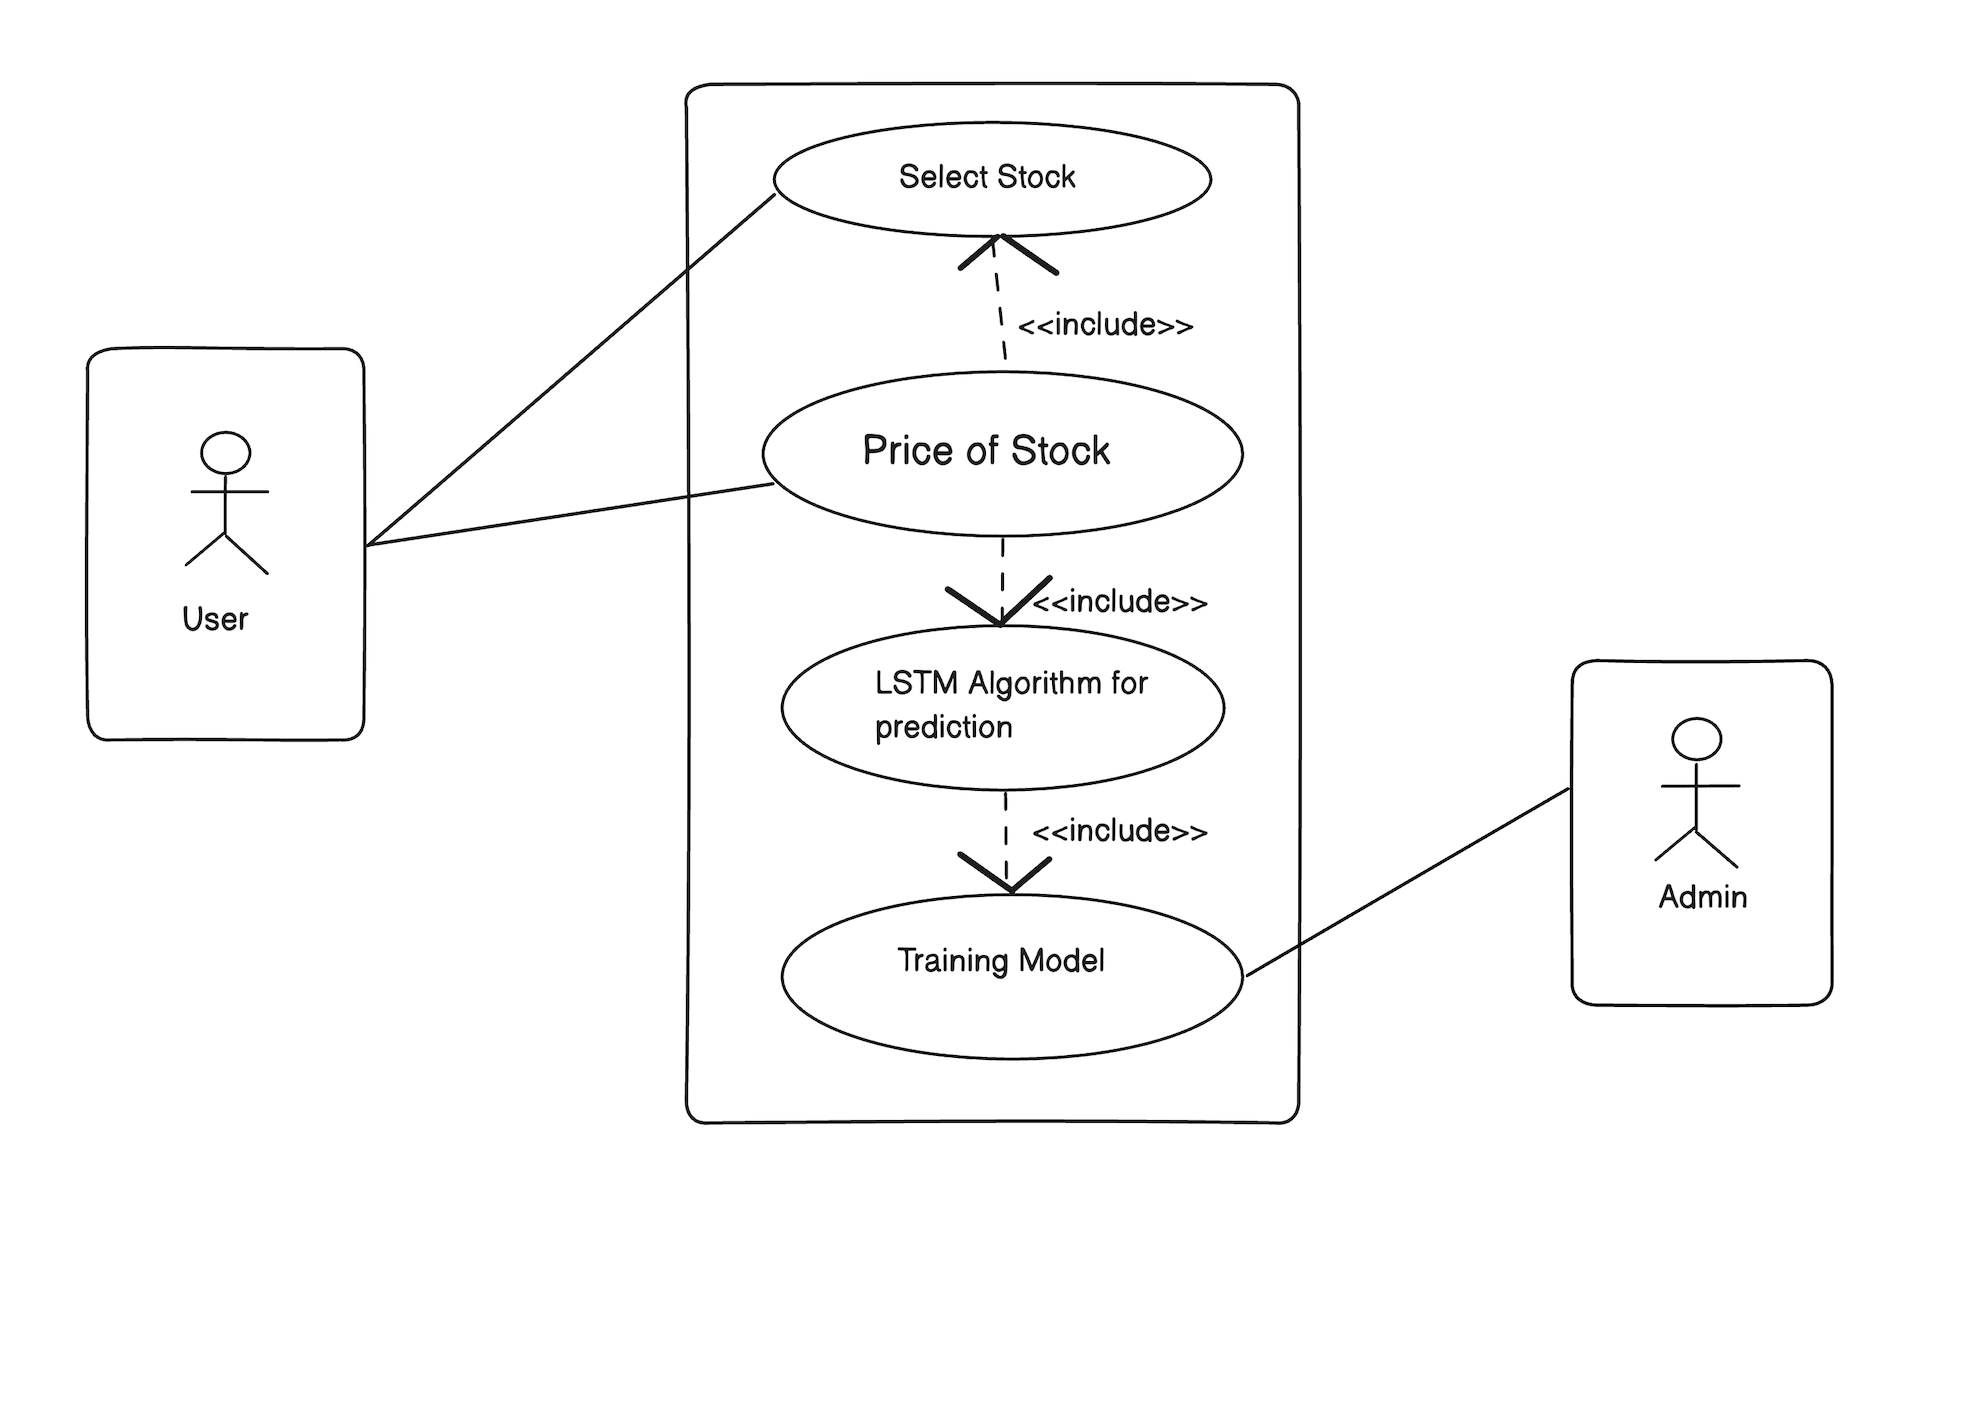
\includegraphics[width=1\textwidth]{Graphics/use_case.png}  
    \caption{Use Case Diagram}
    \label{fig:example}  
\end{figure}
\begin{figure}[h]
    \centering
    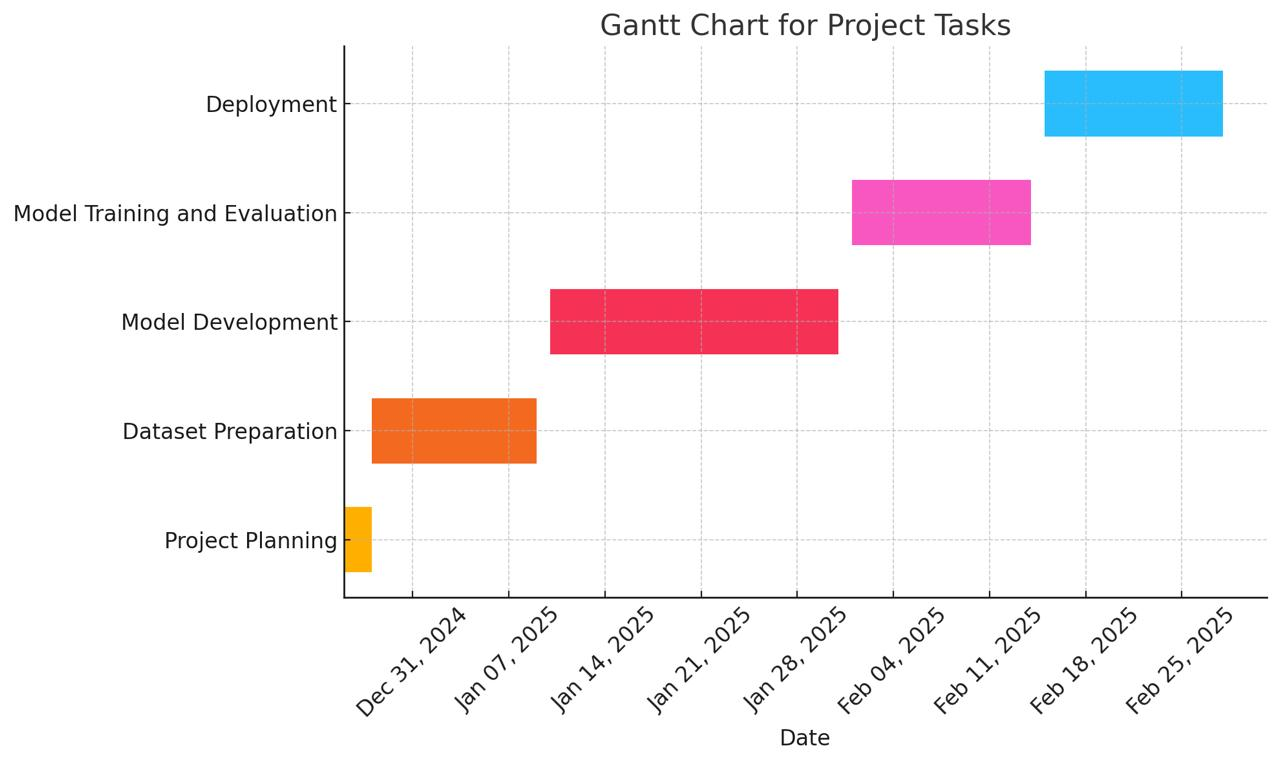
\includegraphics[width=1\textwidth]{Graphics/gantt.jpeg}  
    \caption{Gantt Chart}
    \label{fig:example}  
\end{figure}
\begin{figure}[h]
    \centering
    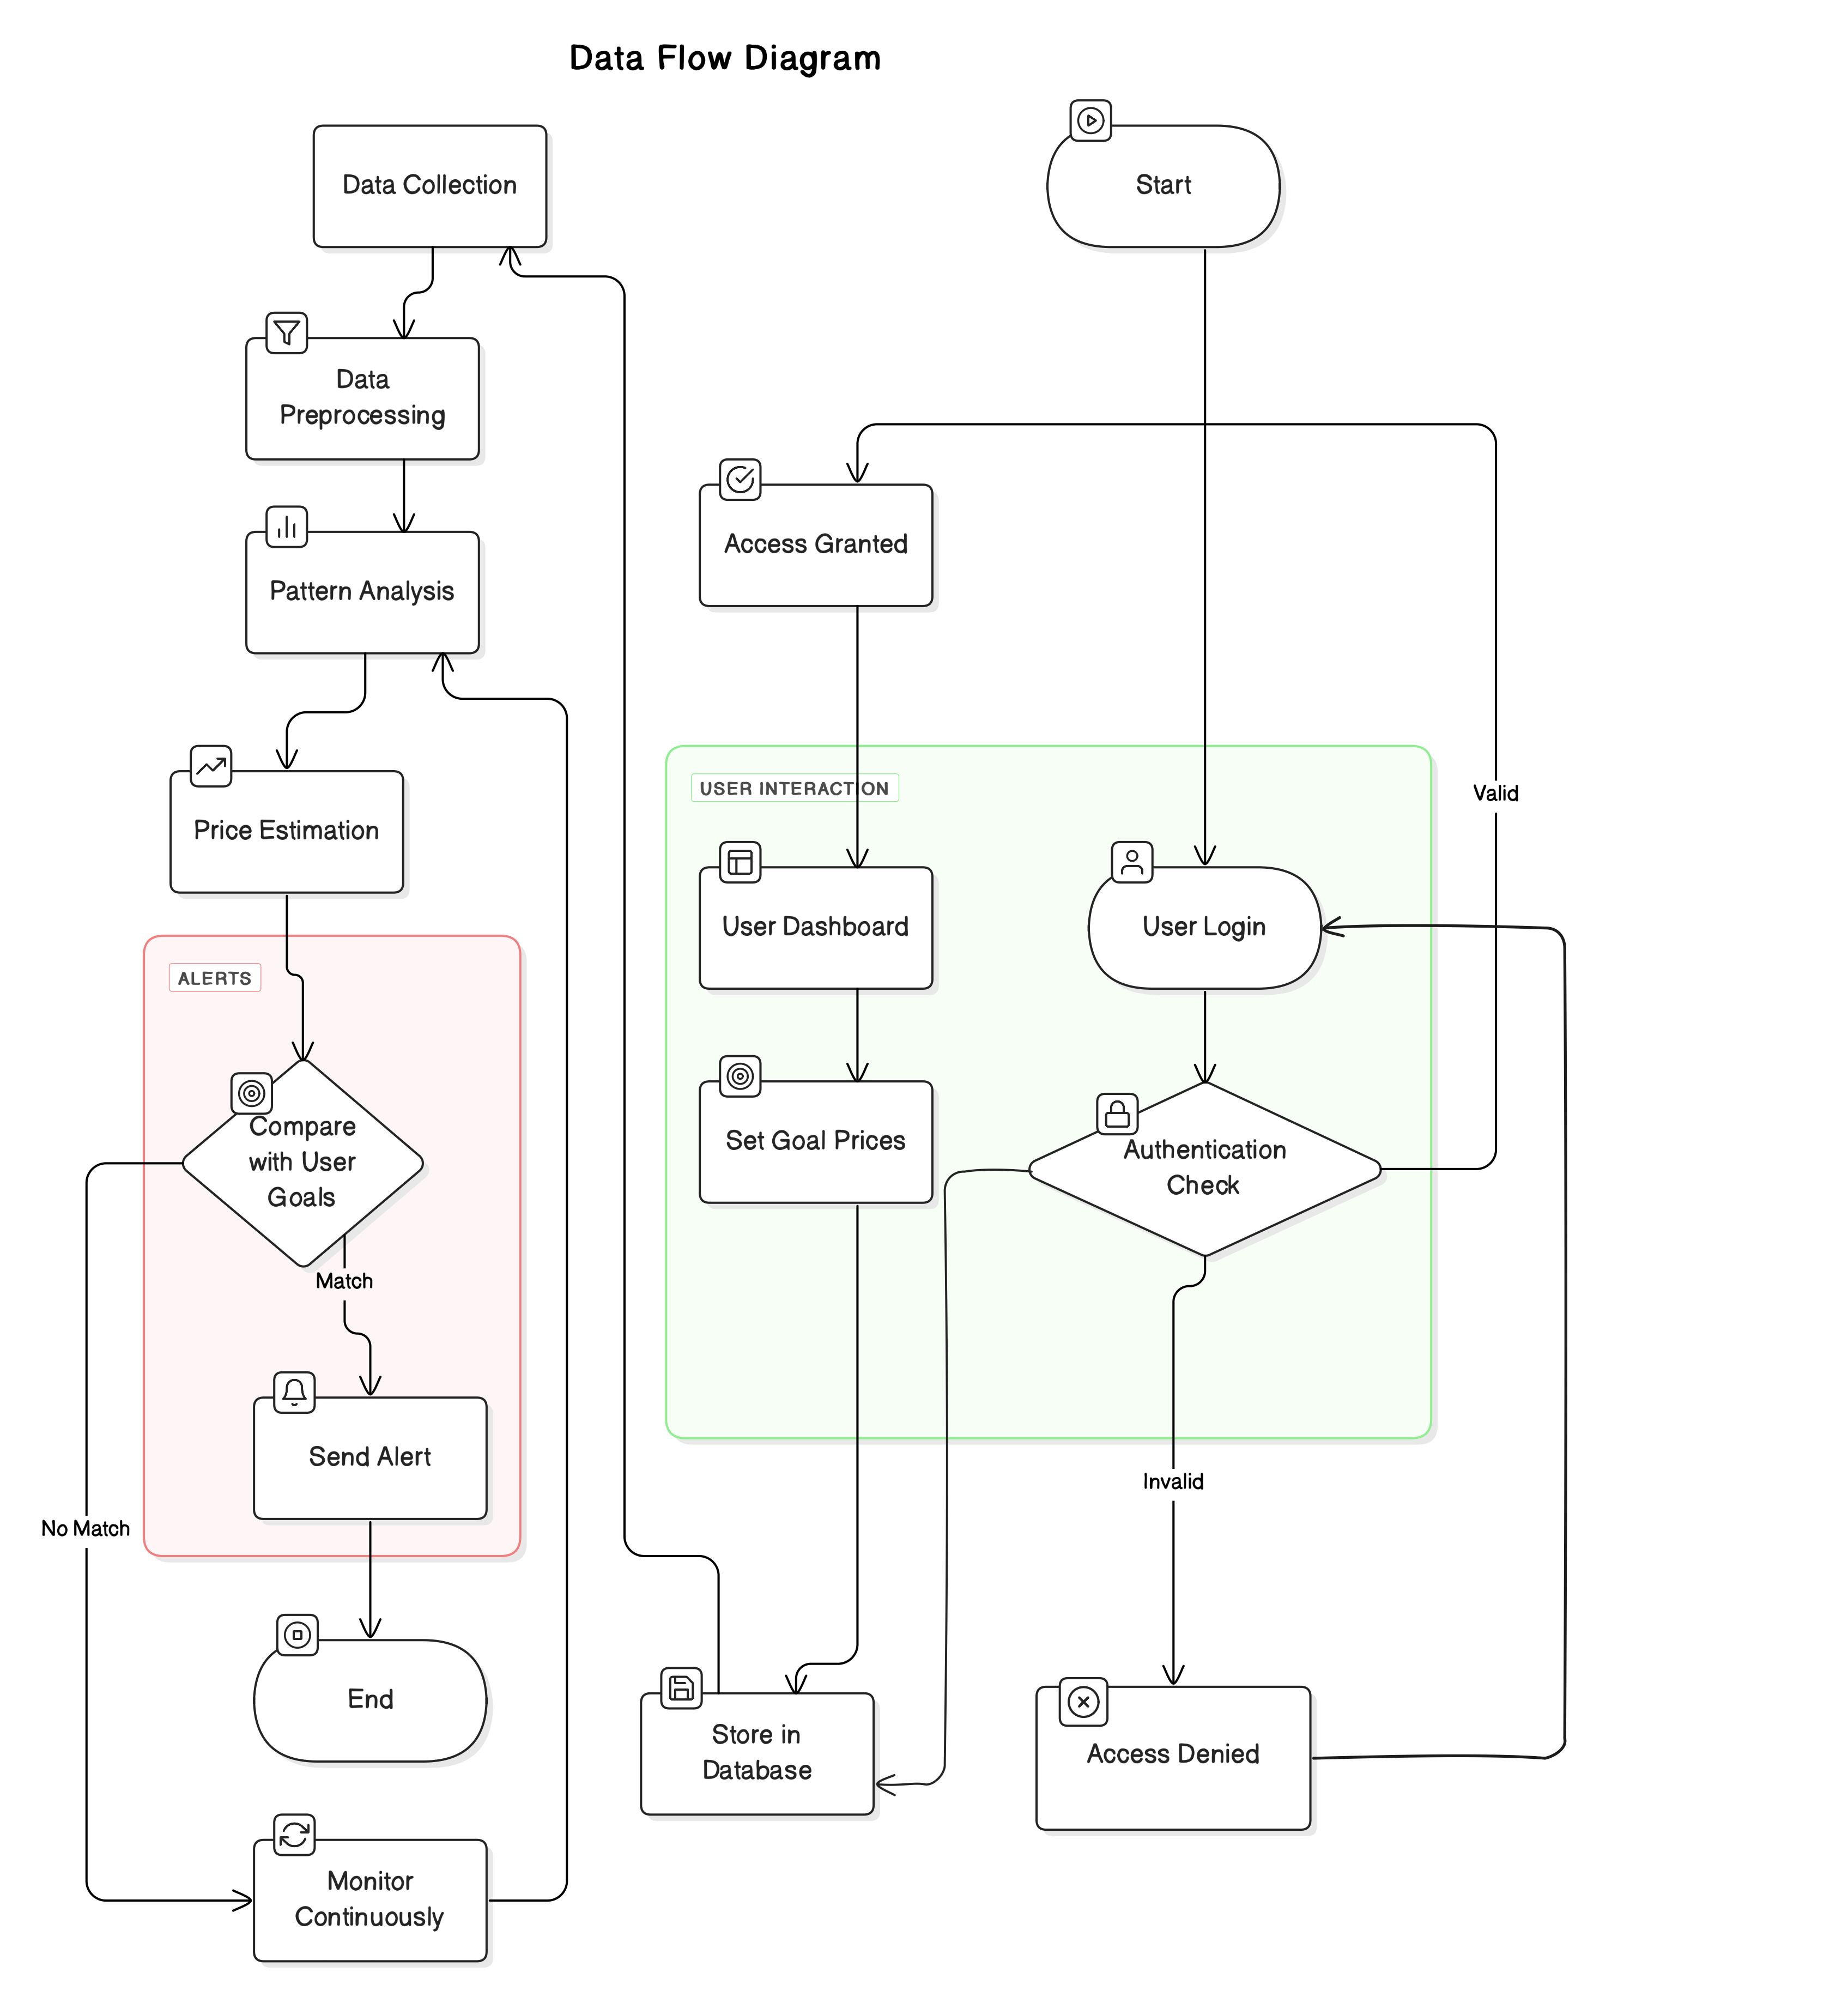
\includegraphics[width=1.2\textwidth]{Graphics/data_flow.png}  
    \caption{Data Flow Diagram}
    \label{fig:example}  
\end{figure}
\begin{figure}
    \centering
    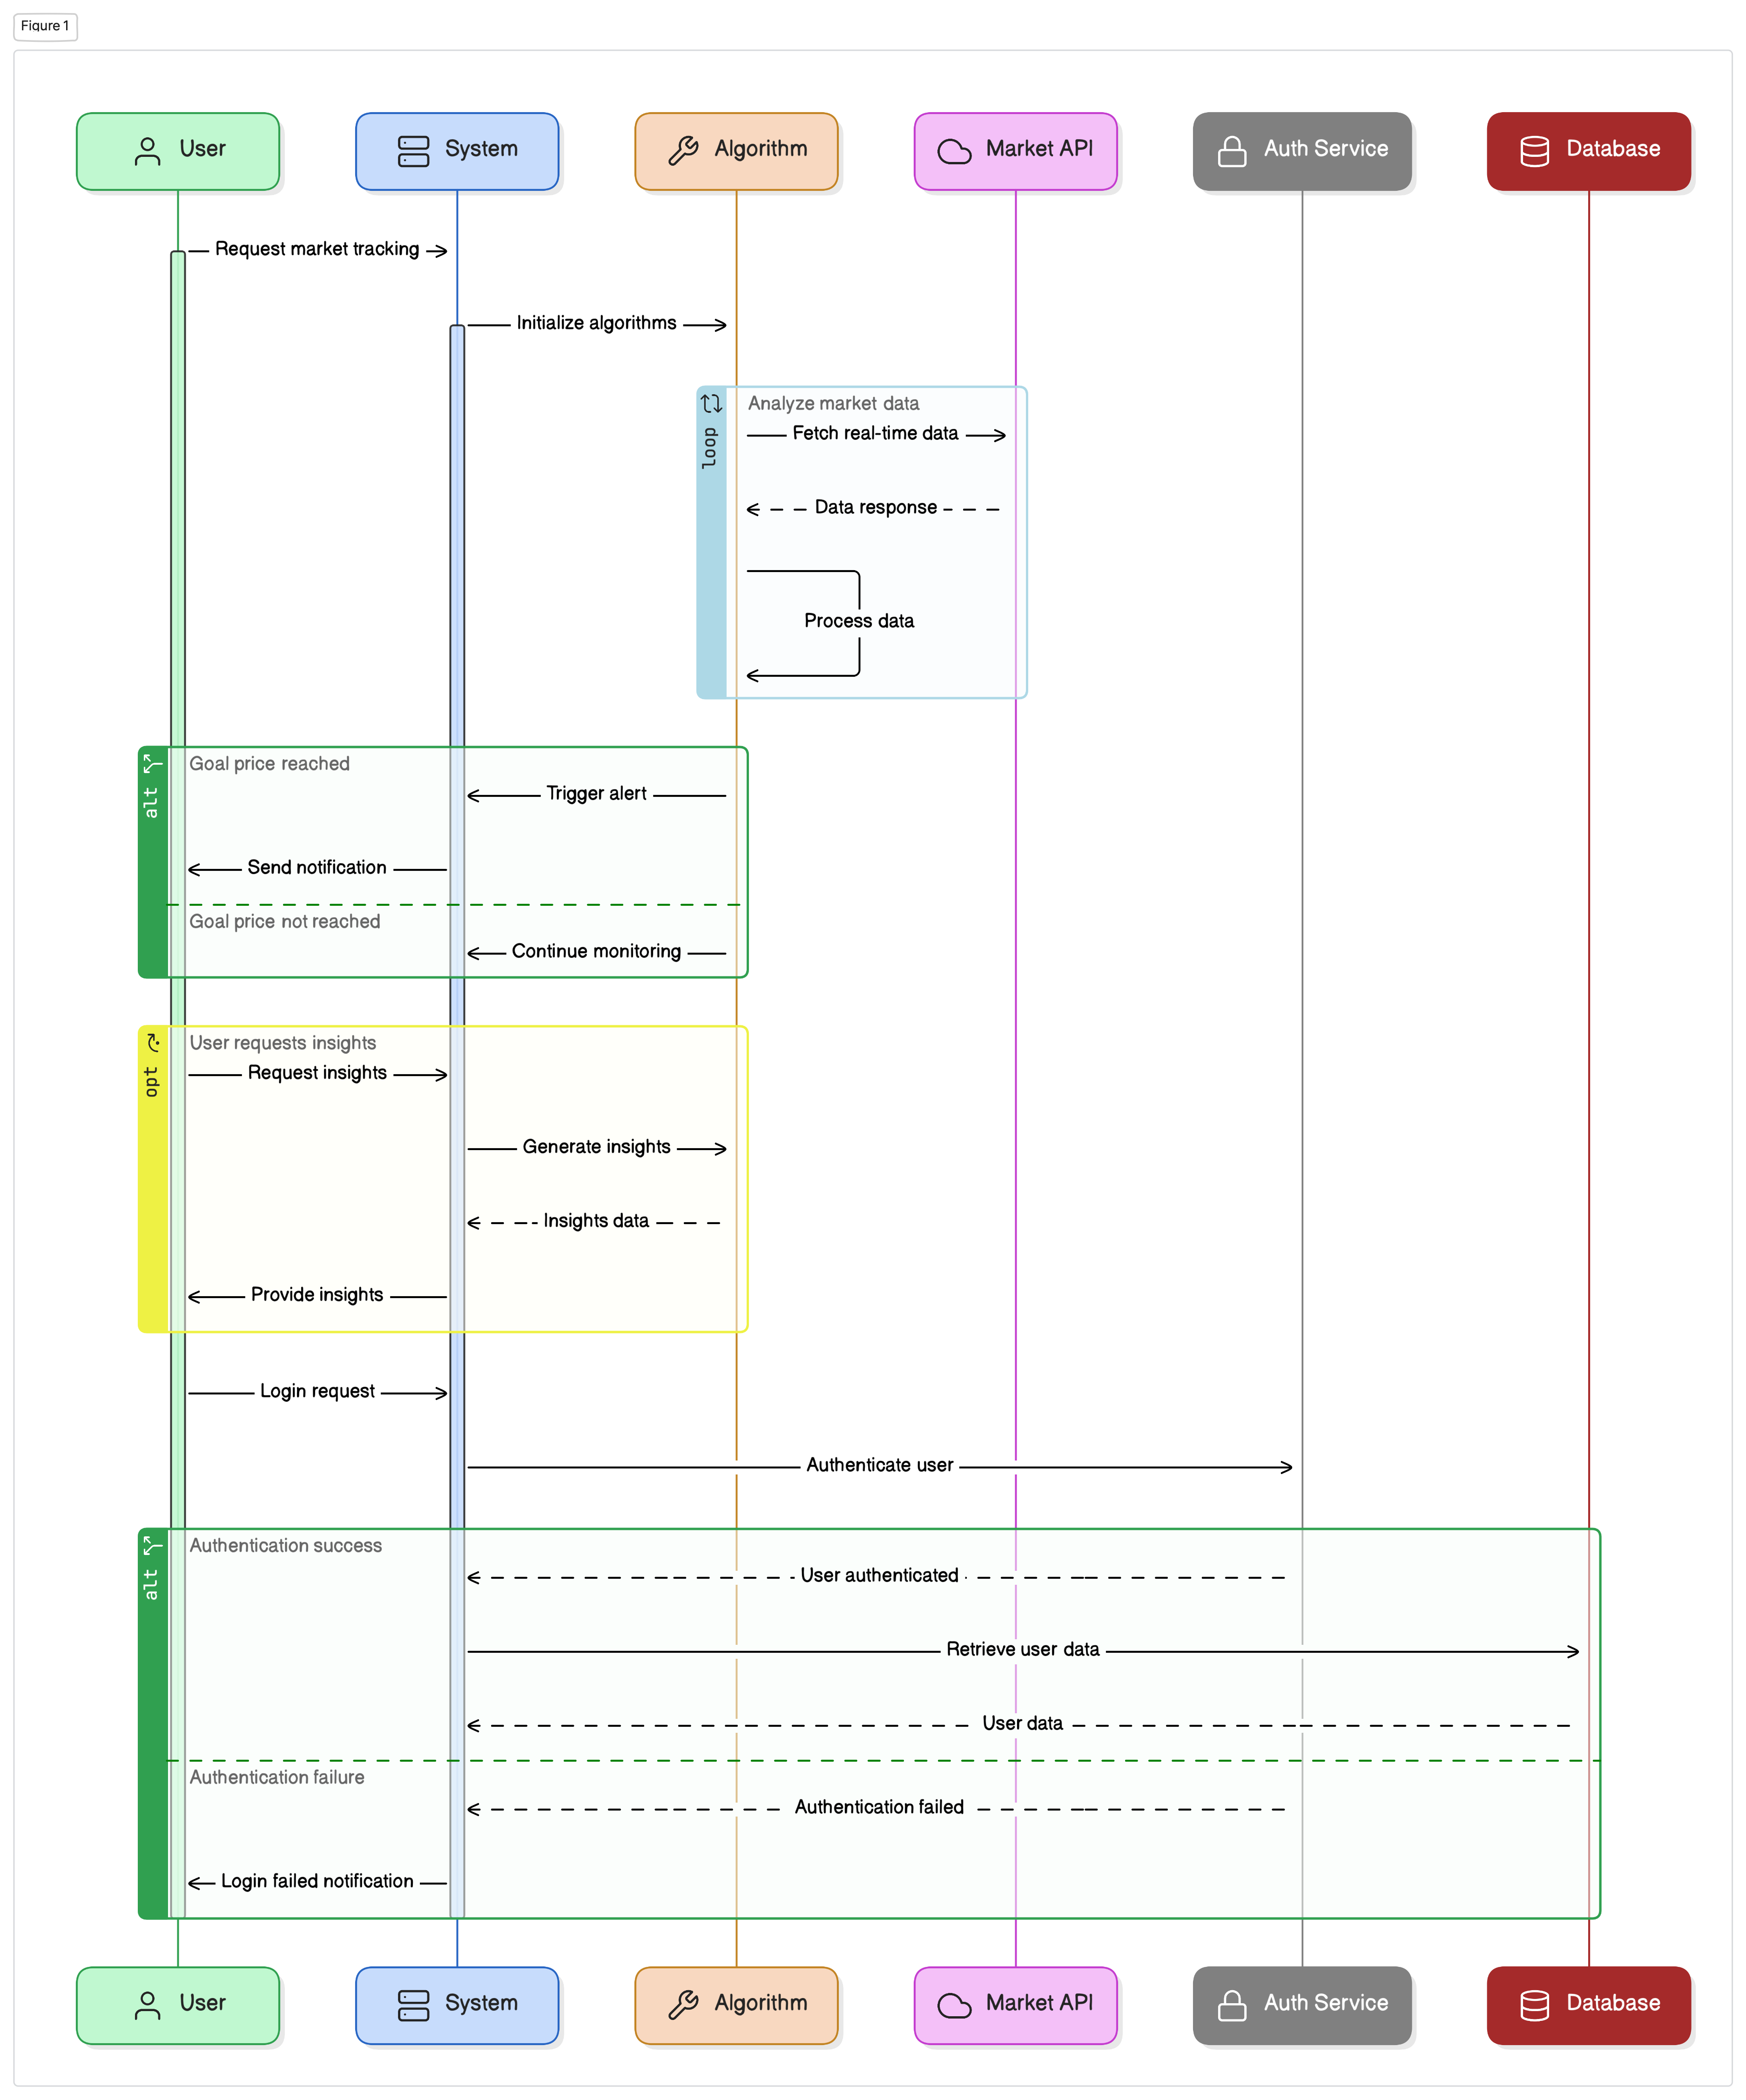
\includegraphics[width=1.1\textwidth]{Graphics/sequence.png}
    \caption{Sequence Diagram}
    \label{fig:enter-label}
\end{figure}
   % \centering
    
   %  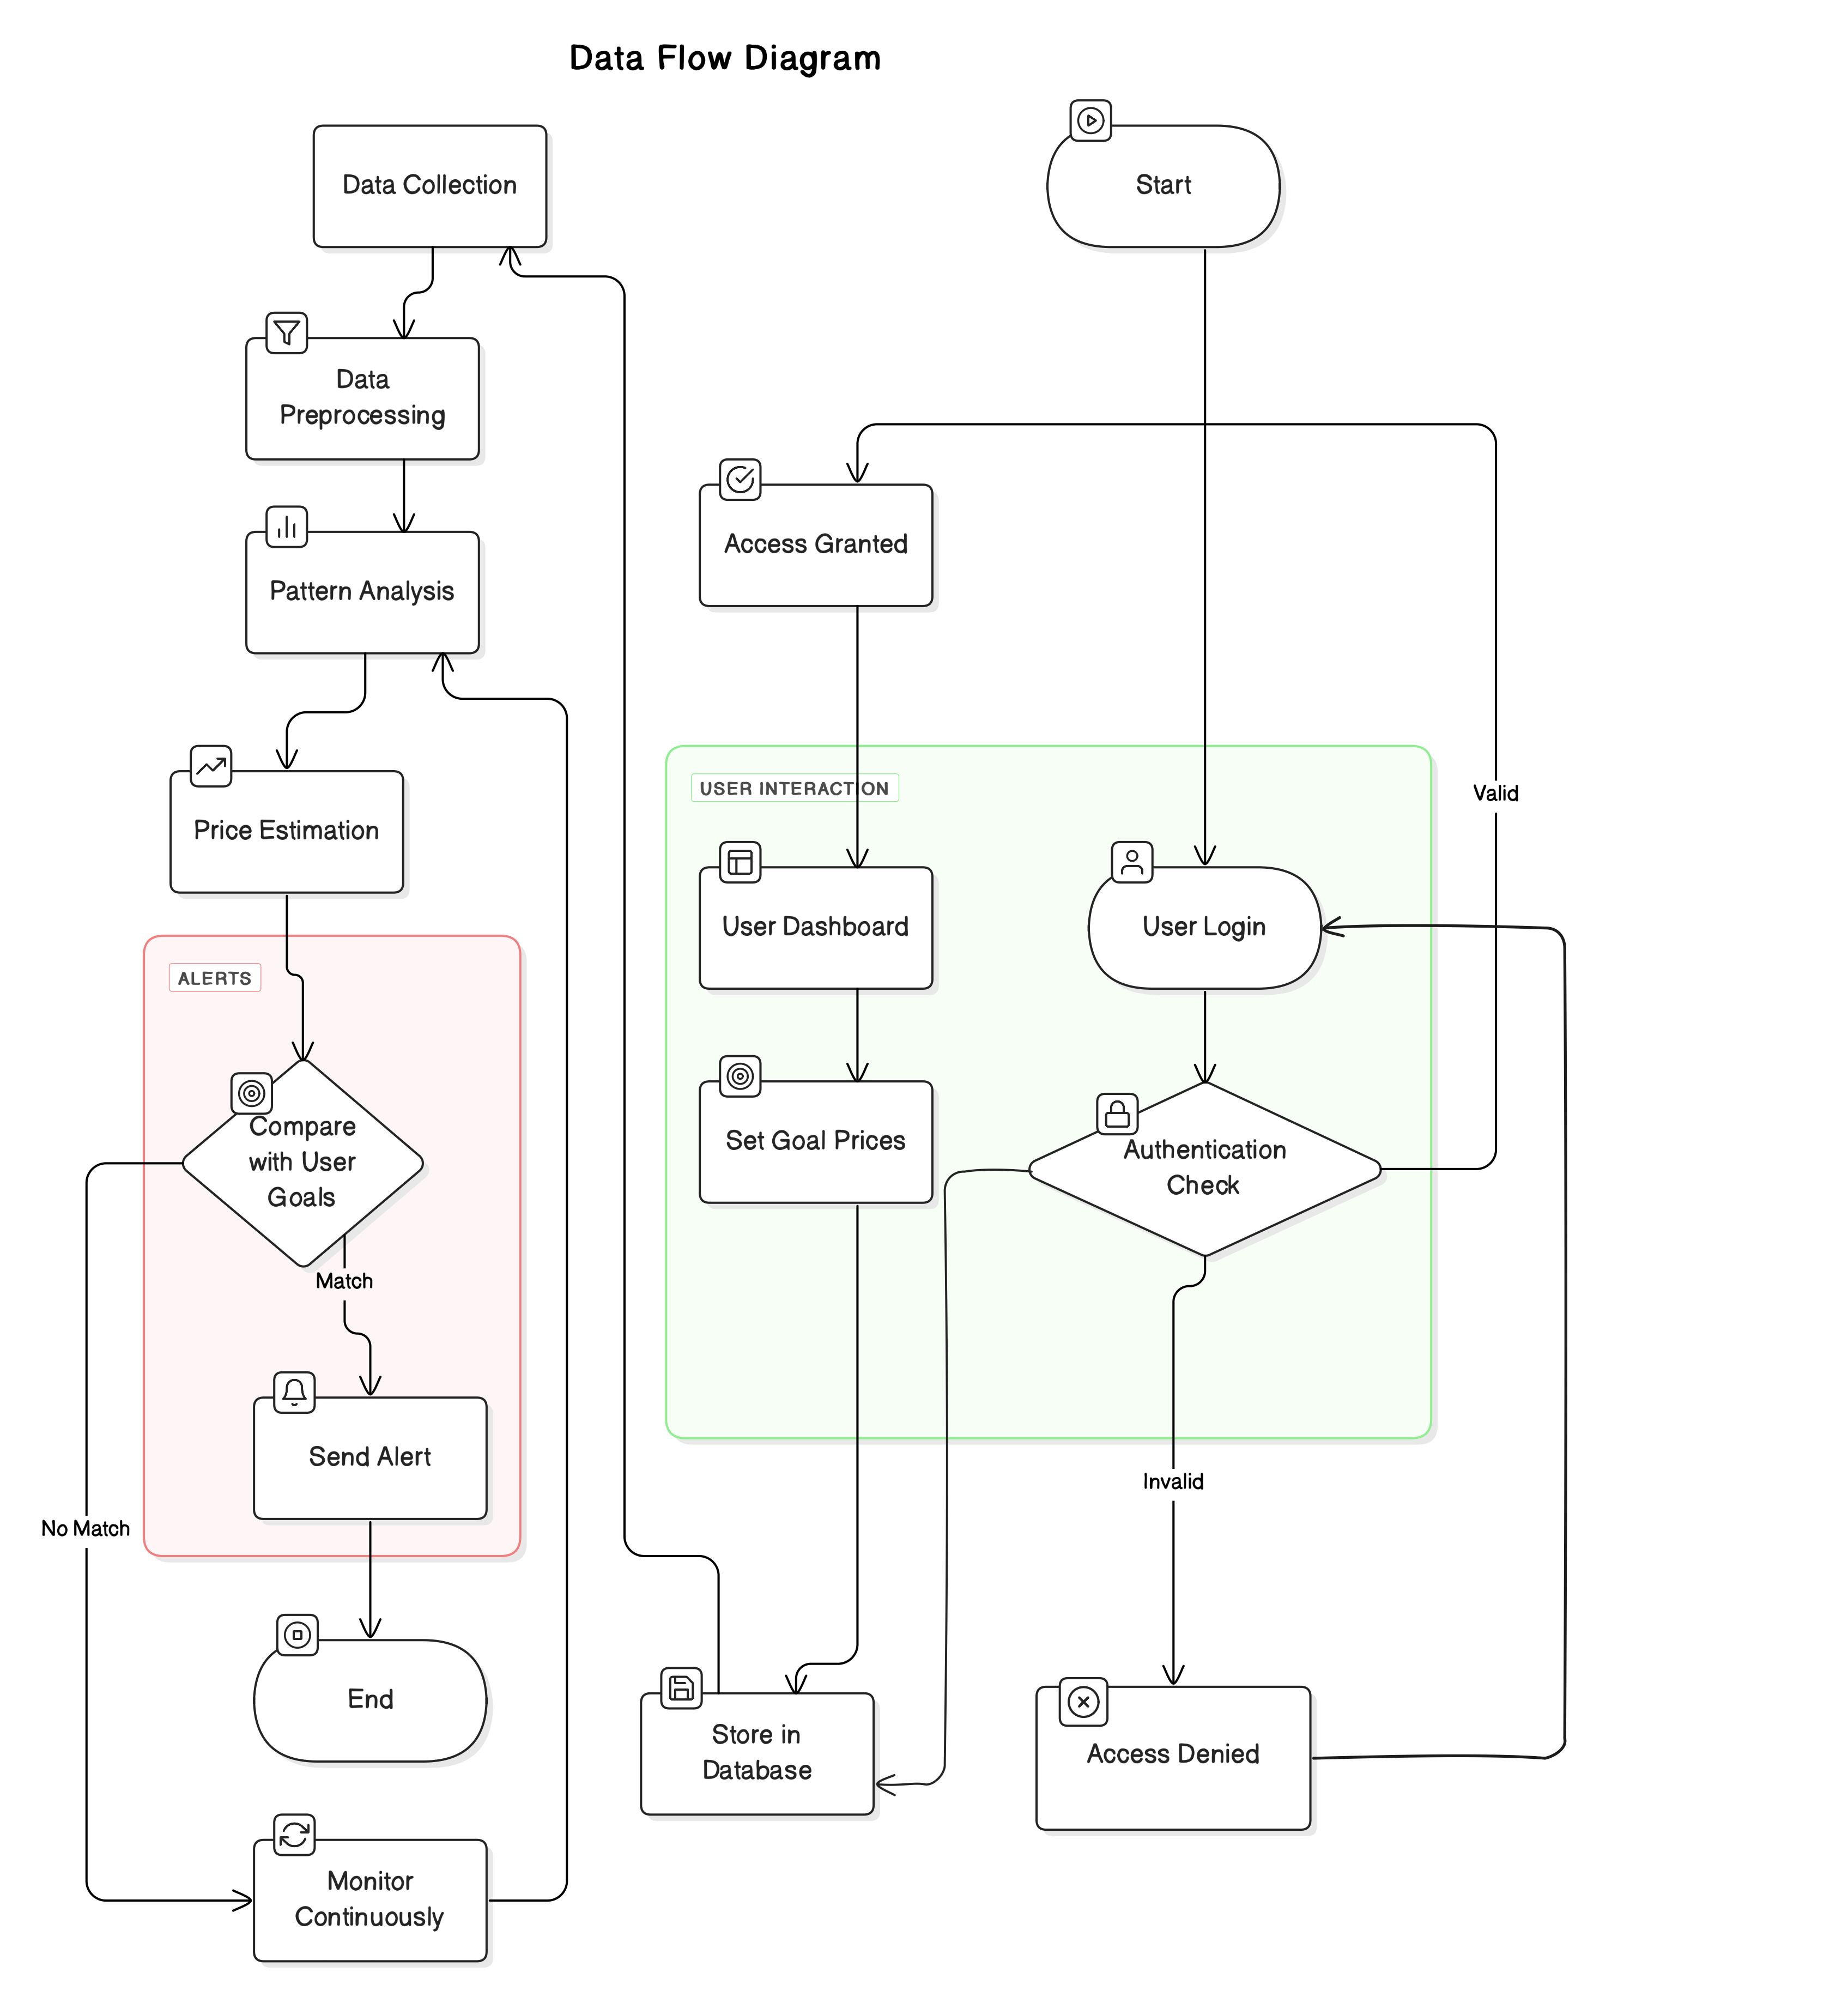
\includegraphics[width=1\textwidth]{Graphics/data_flow.png}\par
   %  \vspace{1.cm}


\chapter{EXPECTED RESULTS}
The expected results of this project are outlined below:

    
\begin{enumerate}

\item \textbf {Accurate stock prediction:}
\begin{itemize}
\item Provide reliable forecasts of stock price movements using machine learning models.
\item Demonstrate model performance through metrics such as Mean Absolute Error (MAE) or Root Mean Squared Error (RMSE).
\end{itemize}

\item  \textbf {Real-Time Stock Tracking:}
\begin{itemize}
\item Successfully fetch and display live stock market data from integrated APIs.
\item Update data with minimal latency to ensure real-time accuracy.

\end{itemize}

\item \textbf {User Goal Notifications:}
\begin{itemize}
 \item Alert users instantly when their defined goal prices are reached.

\item Ensure notifications are delivered through selected channels, such as push notifications or email.
\end{itemize}


\item  \textbf  {Interactive Visualization:}
\begin{itemize}
\item Display clear and intuitive graphs for stock trends, both historical and predicted.

\item Provide dashboards that allow users to monitor multiple stocks and goals simultaneously.

\end{itemize}

\item \textbf {Seamless User Experience:}
\begin{itemize}
\item Ensure an intuitive, responsive interface across devices (mobile, tablet, and desktop).

\item Facilitate smooth interactions for setting goals, viewing predictions, and managing notifications.

\end{itemize}

\end{enumerate}



\addcontentsline{toc}{chapter}{REFERENCES  }
\renewcommand{\bibname}{REFERENCES}
\bibliographystyle{unsrt}
\nocite{*}
\bibliography{references}



\cite{author2024}

\include{Conclusion}
% \addcontentsline{toc}{chapter}{APPENDIX}

\centering{\textbf{APPENDIX A}}
\vspace{1cm}

\vspace{1cm}





\end{document}












